% Drawing 146/04-13 -- folder 146, batch 04, archive page 74 (PDF page 75).
% Transcription: Un triangle sphérique de sommets $0$, $1$, $\infty$, avec un signe $\xi$ (ou $\zeta$) à gauche et un $i$ au-dessous ; à droite, une figure mêlant un triangle (sommets marqués, dont l'un $\infty$ biffé et l'autre $1$) et un pentagone, une région hachurée en zigzag.
% Kind: spherical triangle 0, 1, infinity; triangle and pentagon. Method 2 (schematic redraw from the facsimile). Status: ok.
% Notes: Left: the spherical triangle 0, 1, infinity (two curved sides, one nearly straight), the sign xi (or zeta) at its left and i below, as in the transcription. Right: a triangle (vertices marked, one struck infinity, one 1) with inner lines, a pentagon overlapping it, the zigzag-hatched region between. The inner lines of the triangle are drawn as seen; which of them are struck is not clear.
% Coordinates: 1 unit = 1 mm = 1/100 of the crop width (bbox in page fractions: [0.12, 0.25, 0.72, 0.43]).
% Redrawn by Claude (claude-opus-5-5), issue #73 pilot, 2026-11-07; not checked by a human; not compiled (no TeX in the session).
% Rights: reproduces part of the work -- behind RENDER_TRANSCRIPTS, never published by itself.
\documentclass[tikz,border=3pt]{standalone}
\usepackage{amsmath,amssymb}
\usetikzlibrary{patterns,arrows.meta}
\tikzset{pencil/.style={black!45}, struck/.style={black!35}, mark/.style={circle,draw,inner sep=1.3pt}, pt/.style={circle,fill,inner sep=0.9pt}, opt/.style={circle,draw,fill=white,inner sep=1.1pt}}
\begin{document}
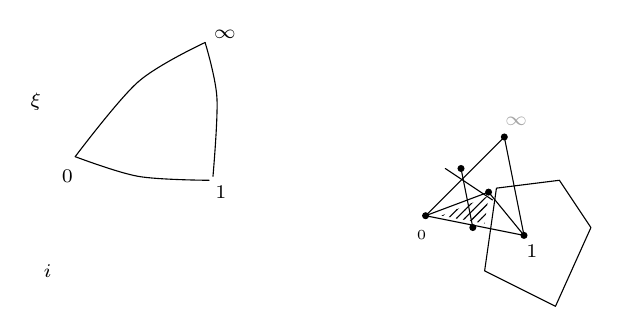
\begin{tikzpicture}[x=1mm,y=1mm,line cap=round,line join=round,font=\scriptsize]
\draw plot[smooth, tension=0.55] coordinates {(27,-19.5) (35,-10) (43.5,-5)};
\draw plot[smooth, tension=0.55] coordinates {(43.5,-5) (45,-12) (44.5,-22)};
\draw plot[smooth, tension=0.55] coordinates {(27,-19.5) (35,-22) (44,-22.5)};
\node[inner sep=1pt] at (26,-22) {\scriptsize $0$};
\node[inner sep=1pt] at (46,-4) {\scriptsize $\infty$};
\node[inner sep=1pt] at (45.5,-24) {\scriptsize $1$};
\node[inner sep=1pt] at (22,-12.5) {\scriptsize $\xi$};
\node[inner sep=1pt] at (23.5,-34) {\scriptsize $i$};
\draw (71.5,-27) -- (81.5,-17) -- (84,-29.5) -- cycle;
\draw (71.5,-27) -- (79.5,-24);
\draw (76,-21) -- (77.5,-28.5);
\draw (79.5,-24) -- (84,-29.5);
\draw (74,-21) -- (80,-25);
\node[pt] at (71.5,-27) {};
\node[pt] at (81.5,-17) {};
\node[pt] at (84,-29.5) {};
\node[pt] at (76,-21) {};
\node[pt] at (77.5,-28.5) {};
\node[pt] at (79.5,-24) {};
\draw (80.5,-23.5) -- (88.5,-22.5) -- (92.5,-28.5) -- (88,-38.5) -- (79,-34) -- cycle;
\fill[pattern=north east lines] (73.5,-27) -- (79.5,-24.5) -- (79,-28) -- cycle;
\node[inner sep=1pt,struck] at (83,-15) {\scriptsize $\infty$};
\node[inner sep=1pt] at (71,-29.5) {\tiny $0$};
\node[inner sep=1pt] at (85,-31.5) {\scriptsize $1$};
\end{tikzpicture}
\end{document}
